\documentclass[11pt, a4paper]{report}
\usepackage{graphicx}
\usepackage[table,xcdraw]{xcolor}
\usepackage{geometry}
\usepackage{float}
\usepackage{authblk}
\usepackage{anyfontsize}
\usepackage[document]{ragged2e}
\usepackage{titlesec}
\usepackage[parfill]{parskip}
\usepackage{color}   %May be necessary if you want to color links
\usepackage{hyperref}
\usepackage{caption}
\usepackage{tabularx}
\usepackage{longtable}
\usepackage{blindtext}
\usepackage{wrapfig}
\hypersetup{
    colorlinks=true, %set true if you want colored links
    linktoc=all,     %set to all if you want both sections and subsections linked
    linkcolor=black,  %choose some color if you want links to stand out
}
\titleformat{\chapter}[hang] 
{\normalfont\huge\bfseries}{\chaptertitlename\ \thechapter:}{1em}{} 
\geometry{left=2.5cm,right=2.5cm,top=2.5cm,bottom=2.5cm}
\graphicspath{ {./images/} }

\begin{document}  
    \pagestyle{empty}
\centering
\fontsize{2cm}{2cm}\selectfont{Module Design Document} \\
\vspace{2mm}
\fontsize{1cm}{1cm}\selectfont Audio digital signal processor \\
\vspace{2mm}
\large BeCreative Minor\\
\normalsize
\vspace{4cm}
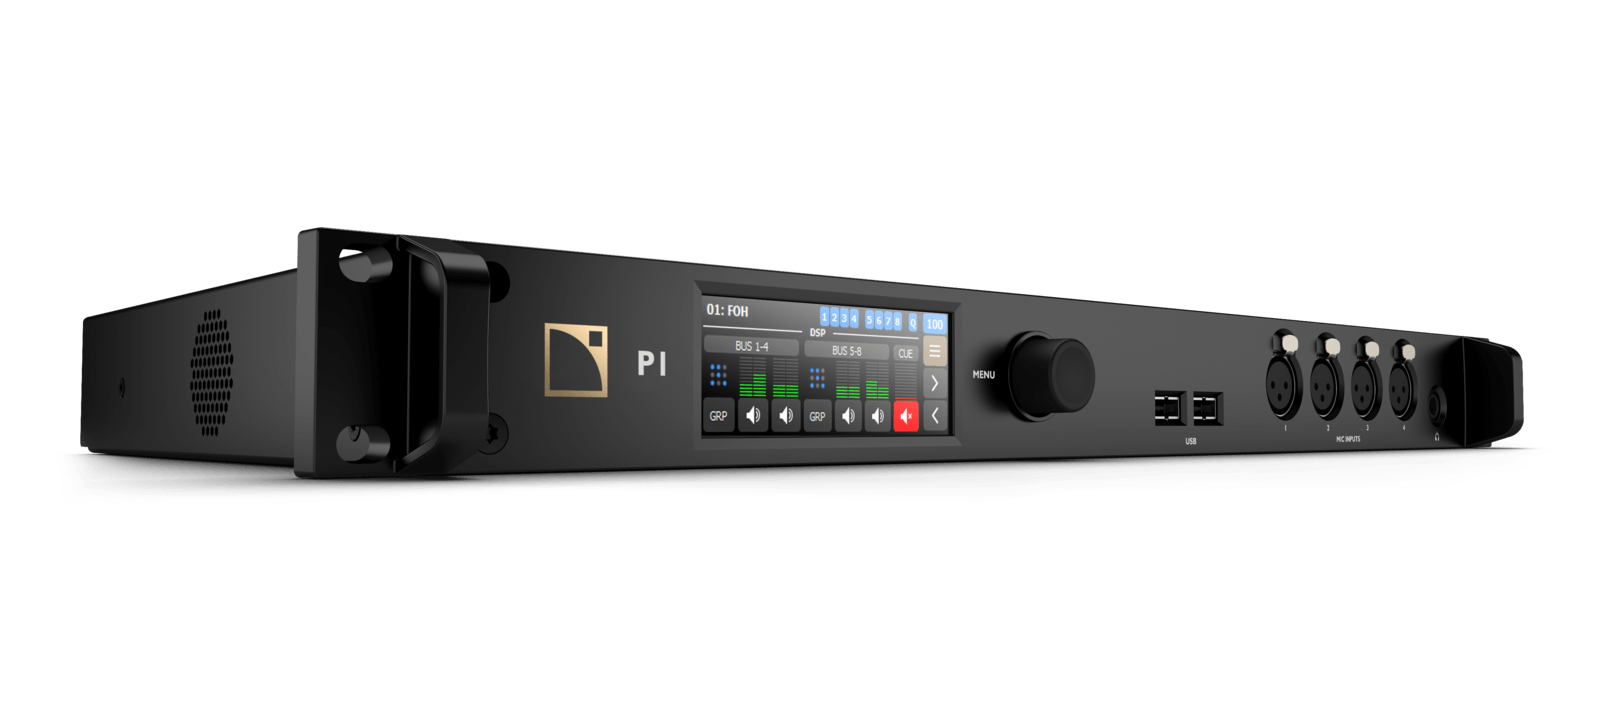
\includegraphics[width=\linewidth]{3DR_P1_Perspective.png}\\
\vfill
\normalsize Busse Lommers \\
Robin van den Dungen \\
Mahmud Gürler \\
Silas Kamphuis \\
Hein Verhallen \\
Youri Tils \\
Fontys Hogescholen, De Rondom 1, 5612 AP Eindhoven \\
\today

\begin{justify}

\chapter*{Summary}
The following text translates to English as:

This report describes how this project group created an audio DSP for the BeCreative Minor. This was done because the members of the group wanted to learn more about it and improve their technical knowledge.

Chapter "Problem Description" outlines the project's background and goals. Chapter "Research" describes the preliminary investigations conducted. Chapter "Concept Development" explains how the product concept was developed. Chapter "Realization" details the actual design of the audio DSP. Chapter "Verification" discusses the product testing process. Finally, in chapters "Conclusions" and "Recommendations," the conclusion and recommendations are respectively described.

\newpage
\tableofcontents
\thispagestyle{empty}

\listoffigures
\thispagestyle{empty}

\listoftables
\thispagestyle{empty}

\newpage
\pagestyle{plain}

\chapter*{Report contribution}	%Fill-in only regarding the report contribution.
\begin{longtable}{|c|c|c|}
	\hline
	\textbf{Chapter} & \textbf{Paragraph} & \textbf{Person} \\ \hline
	Problem Description			& Background					& All	 					\\ \hline
	Introduction				& NA							& Busse 					\\ \hline
								& Problem description			& Robin						\\ \hline
								& Project goals					& All						\\ \hline
								& Requirements					& All 						\\ \hline
								& Project scope					& All 						\\ \hline
								& Boundary condition			& All						\\ \hline
								& Project approach				& All						\\ \hline
								& Verification method			& All						\\ \hline
	Research 					& Research objectives			& All 						\\ \hline
								& Research questions			& All 						\\ \hline
								& Research approach				& All 						\\ \hline
								& Results						& All 						\\ \hline
	Concept Development 		& Concept overview				& Youri						\\ \hline
								& Front-end						& Silas						\\ \hline
								& Audio-DSP						& Youri						\\ \hline
								& Back-end						& Silas						\\ \hline
								& Interfacing					& Robin						\\ \hline
								& Front-end						& Robin						\\ \hline
								& Audio-DSP						& Youri						\\ \hline
								& Back-end						& Robin						\\ \hline
								& Power supplies				& Mahmud \& Robin			\\ \hline
								& Modules						& Busse						\\ \hline
								& UI							& Hein \& Busse				\\ \hline
								& Hardware programming			& Busse						\\ \hline
								& Hardware design				& Busse						\\ \hline
								& Design decissions				& Busse						\\ \hline
	Realization					& Hardware						& NA						\\ \hline
								& Schematic						& Robin						\\ \hline
								& Printed circuit board			& Silas						\\ \hline
								& Case							& Busse						\\ \hline
								& Firmware						& Youri						\\ \hline
								& I2S decoder and encoder		& Youri						\\ \hline
								& I2C controller				& Youri						\\ \hline
								& Band-pass filter				& Youri						\\ \hline
								& Sinewave generator			& Youri						\\ \hline
								& Effects						& Youri \& Busse			\\ \hline
								& User interface				& Hein \& Busse				\\ \hline
								& User interface				& Hein \& Busse				\\ \hline
	Verification				& Method						& Robin						\\ \hline
								& Hardware						& Mahmud \& Robin			\\ \hline
								& Firmware						& Youri						\\ \hline
								& Results						& NA						\\ \hline
								& Hardware						& Mahmud					\\ \hline
								& Firmware						& Youri						\\ \hline
								& Conclusions					& Mahmud \& Silas \& Robin 	\\ \hline
								& Hardware						& Mahmud					\\ \hline
								& Firmware						& Youri						\\ \hline
	Conclusions					& NA							& Silas						\\ \hline
	Recommendations				& NA							& Silas						\\ \hline
	Summary						& NA							& Robin						\\ \hline
	Bibliography				& NA							& Busse						\\ \hline
	Appendix A: State-space		& NA							& Youri						\\ \hline
	Appendix B: VHDL code		& I2S decoder					& Youri						\\ \hline
								& I2S encoder					& Youri						\\ \hline
								& I2C master					& Youri						\\ \hline
								& State-space BPF code			& Youri						\\ \hline
								& Sinewave generator code		& Youri						\\ \hline
	Appendix C: Schematics		& Buck converter schematic		& Mahmud					\\ \hline
								& SEPIC schematic				& Silas						\\ \hline
								& Linear regulator schematic	& Silas	\& Robin			\\ \hline
								& Main board schematic			& Robin						\\ \hline
								& Buck converter calculations	& Silas						\\ \hline
								& SEPIC calculations			& Robin						\\ \hline
	Appendix D: UI design		& Main menu						& Busse						\\ \hline
								& Adjust preset menu			& Busse						\\ \hline
	Appendix E: Case			& Top view						& Busse						\\ \hline
								& Front view					& Busse						\\ \hline
								& Rear view						& Busse						\\ \hline
	Appendix F: Verification	& Ground spring					& Robin						\\ \hline

	\caption{Revision list of the document}
	\label{table:revision_history}
\end{longtable}

\newpage
\pagestyle{plain}
\setcounter{page}{1}

\chapter*{Abbreviation List}

\begin{table}[!h]
	\centering
	\begin{tabular}{|c|c|}
		\hline
		\textbf{Abbreviation} & \textbf{Explanation}	\\ \hline
		DSP 					& Digital Signal Processor    				\\ \hline
		ADC 					& Analog-to-Digital Converter 				\\ \hline
		BPF 					& Band-Pass Filter							\\ \hline
		CH 						& Channel									\\ \hline
		DAC 					& Digital-to-Analog Converter 				\\ \hline
		FFT 					& Fast Fourier Transform					\\ \hline
		FPGA 					& Field programmable gate array 			\\ \hline
		GBW 					& Gain Bandwidth Product 					\\ \hline
		RAM 					& Random Access Memory	    				\\ \hline
		SEPIC        			& Single-Ended Primary-Inductor Converter	\\ \hline
		SINAD 					& Signal to noise and distortion 			\\ \hline
		TRS 					& Tip ring sleeve connector (jack) 			\\ \hline
	\end{tabular}
	\caption{List of commonly used Abbreviations}
	\label{table:Abbreviation list}
\end{table}
    
    \chapter{Background}
    %BACKGROUND
When listening to music it is of great importance that the speakers are tuned to the environment and the position of the listener. This is necessary to achieve the best experience. If the speakers are not correctly tuned to the surrounding environment, a digital signal processor (DSP) is used to correct this. A DSP is a specialized processor which is used for digital signal processing. 

\noindent In the audio world a DSP is used to optimize a sound system. For example some speakers have some imperfections and a DSP can be used to correct for these imperfections. It is also often used to add more dynamics to sound.


    \chapter{System context design}
    
\begin{figure}[h]
    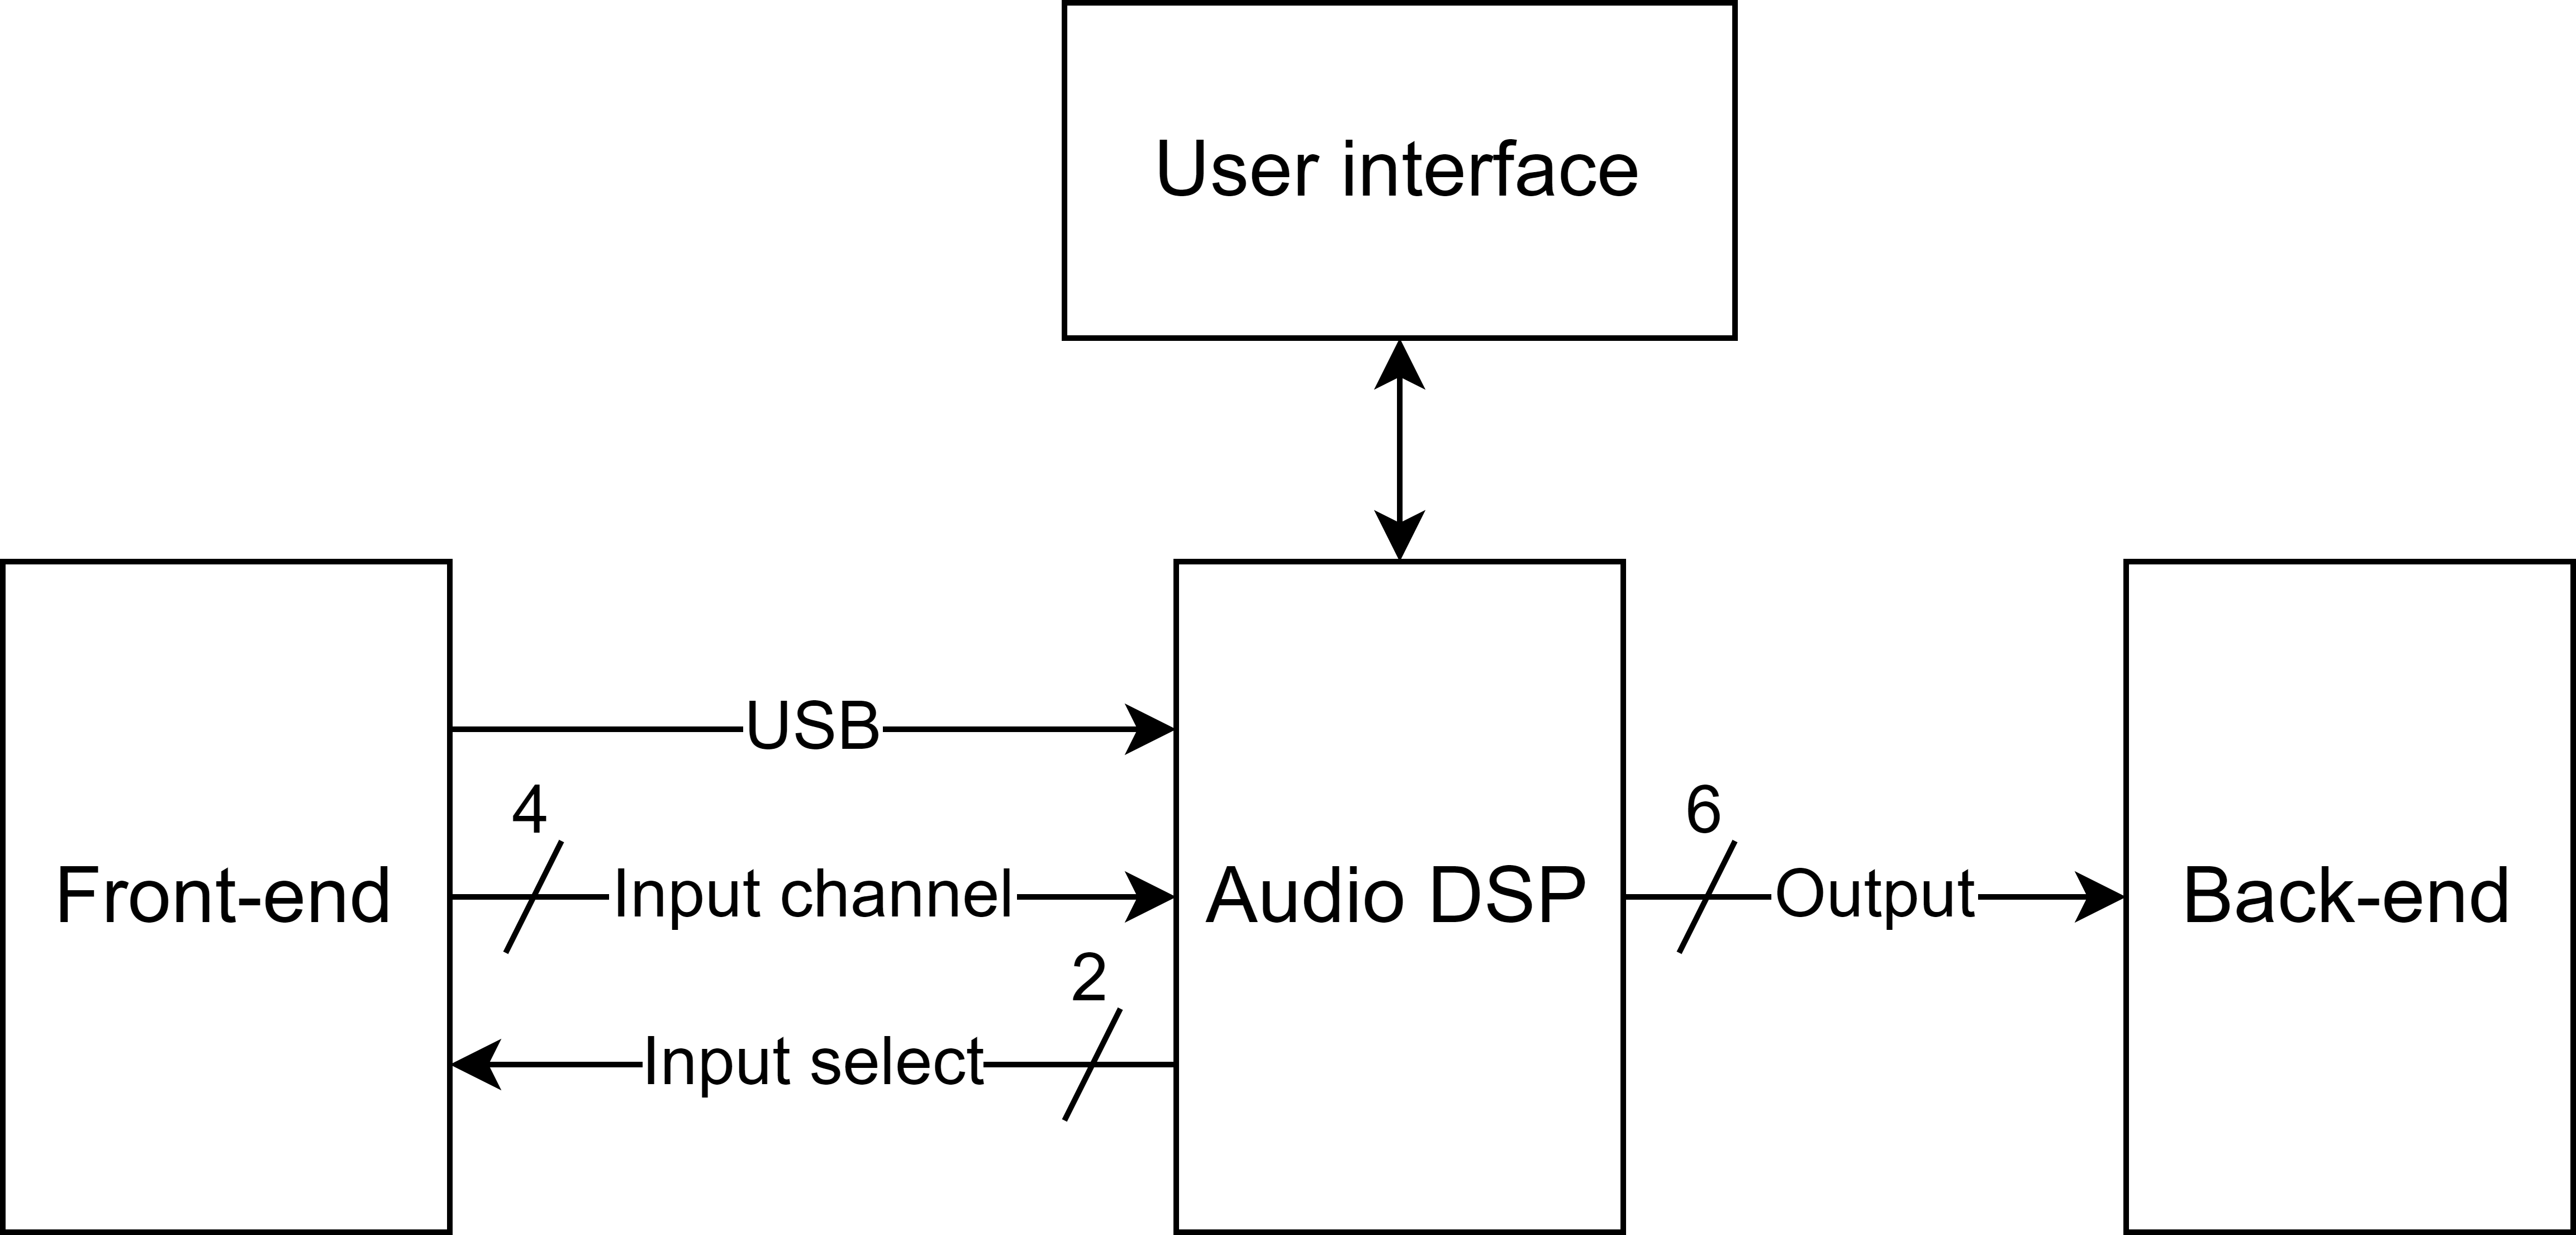
\includegraphics[width=\linewidth]{System context-top level.png}
    \caption{System context diagram of the top-level}
\end{figure}

\section{Front-end}
\begin{figure}[h]
    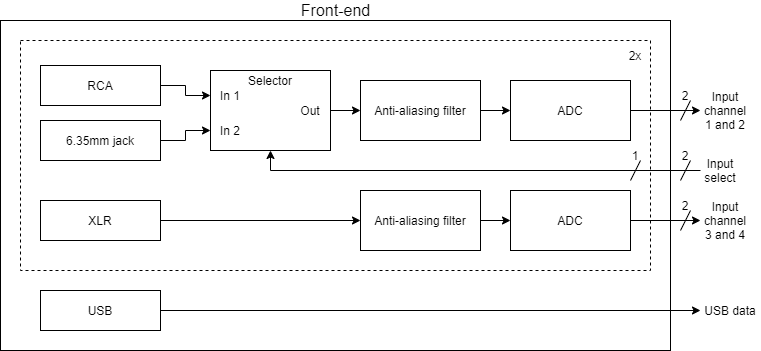
\includegraphics[width=\linewidth]{System context-front-end.png}
    \caption{System context diagram of front-end design}
\end{figure}

\section{Audio-DSP}
\begin{figure}[h]
    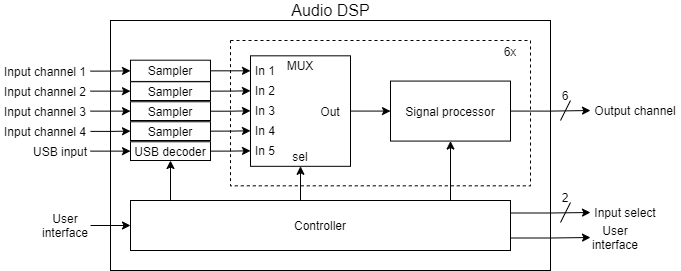
\includegraphics[width=\linewidth]{System context-audio DSP.png}
    \caption{System context diagram of Audio-DSP}
\end{figure}

\section{Back-end}
\begin{figure}[h]
    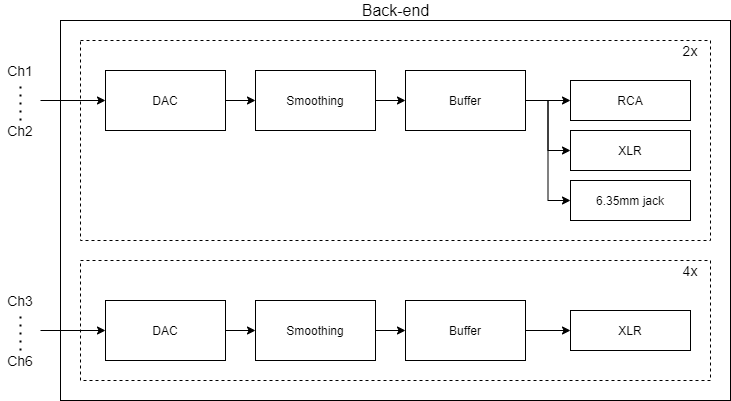
\includegraphics[width=\linewidth]{System context-back-end.png}
    \caption{System context diagram of back-end}
\end{figure}

\section{User interface}


    \chapter{System Architecture}
    The lower level design of the system are explained in the architecture design of the system. 

\section{Audio-DSP}
\begin{figure}[ht]
    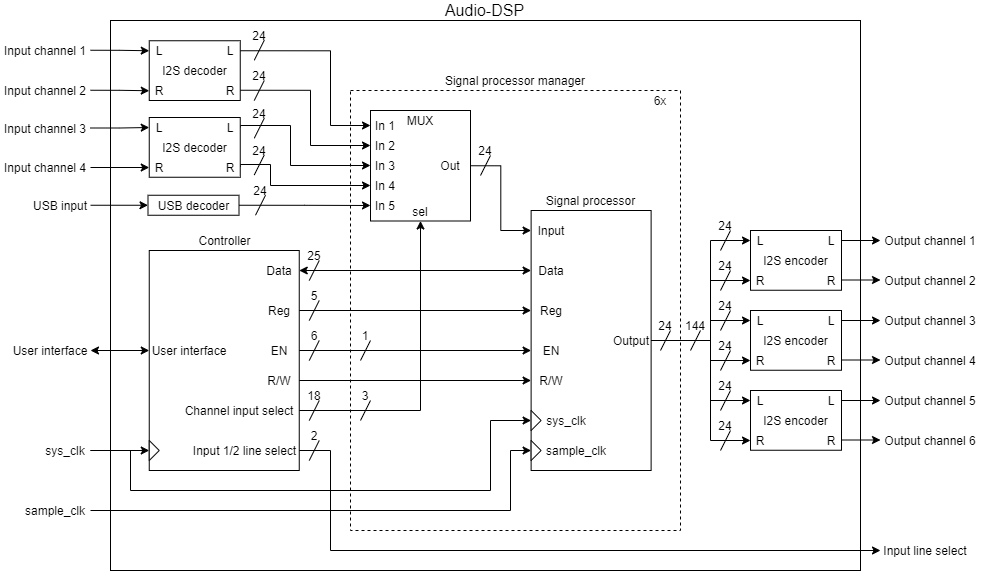
\includegraphics[width=\linewidth]{Audio-DSP architecture.png}\\    
    \caption{Top-level architecture of audio-DSP}
    \label{fig:arch-top}
\end{figure}

In figure \ref*{fig:arch-top} you see the architecture design of the Audio-DSP. Compared to the system context diagram of the Audio-DSP the block is now much more detailed. For instance the input samplers are replaced by $I^2S$ decoders and the output signals are now encoded to $I^2S$. Because most ADCs and DACs use the $I^2S$ protocol to transfer audio data it has been chosen to use the $I^2S$ protocol. The $I^2S$ encoders and decoders each have a left and right input and output. This is because the $I^2S$ protocol transfers a stereo audio signal. But this system uses mono signals. Therefore the system inputs the mono signals on the left and right inputs. This gives the system the ability to transfer two audio channels via one $I^2S$ bus.

The MUX in each of the signal processor managers is controlled via a 3-bit select line. This select line comes from the controller. For the controller to be able to handle all the multiplexers in each signal processor manager, 3-bits $\cdot$ 6 channels = 18 bits are needed. To select the RCA or 6.35mm jack input a 2-bit select line is used.

In order for the signal processor to modify the signal with various digital effects, memory is needed. This memory is stored inside the signal processor block itself. To access and modify the memory some kind of communication protocol had to be chosen in order for the controller to configure the effect parameters. For this a register based memory has been chosen.

Looking at the system requirements it is known that the user is able to adjust the position of each effect in the effects loop. Therefore the signal processor needs registers to store the position of each effect. The system must support at least five effects and should support at least twenty effects. Thus in order to fulfill all the requirements the signal processor should be able to position twenty effects. For this we would need at least 5 bits at each position. The various effects available to the user have configurable parameters. Therefore each effect also needs a register in the signal processor block. Also the equalizer settings are adjustable by the user. This means the equalizer also has a register with data.

The size of the registers can be very large. But to make the communication to the signal processor intuitive the registers will be limited to a maximum amount of bits. In order to choose the most efficient register size the registers should use most of its bits. The size of the register is of no importance for the effect and equalizer parameters as the size only affects the resolution of the parameters. But for the position register 5-bits per position are needed. Thus the register should be dividable by 5 in order to use the most of the registers bits. As there are 20 positions it is chosen to have four position registers with 5 positions (see figure \ref{fig:reg-position}).
This means the register size will be 25 bits.

% \begin{wrapfigure}[20]{r}{0.25\textwidth}
%     \centering
%     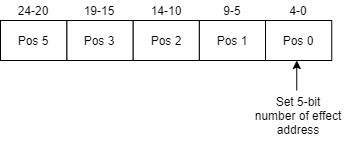
\includegraphics[width=0.25\textwidth]{Position register design}
%     \caption{Effect loop position 0 to 4 register}
%     \label{fig:reg-position}
% \end{wrapfigure}

\begin{figure}[ht]
    \centering
    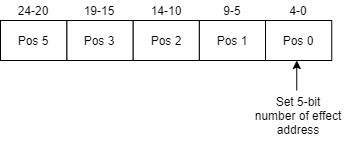
\includegraphics[width=0.4\textwidth]{Position register design}
    \caption{Effect loop position 0 to 4 register}
    \label{fig:reg-position}
\end{figure}

Now that the register size has been defined we need to define the amount of registers needed. The system has 20 effects, therefore 20 effect parameter registers. Each effect needs to be positioned in the position registers which there are four of. Then the equalizer and volume registers are left. when using 5 bits for selecting the registers we would be able to access up to 32 registers. This means that there are $32 - (20 + 4) = 8$ registers left for the equalizer and volume parameters. That is more than enough for these registers.

Thus the data bus will be 25 bits and the register selector line will be 5 bits. With these two lines every register can be accessed by the controller. Now the memory needs to know if the data needs to be read or written. This is indicated by the R/W signal. When this signal is low the memory will be written and when the signal is high the memory will be read.

It is undesired that every signal processor memory will be read or written constantly. Therefore each signal processor block has an enable. When this enable signal is high the memory can be read or written. This gives the controller the ability to read or write to only one signal processor memory at a time. And the ability to write multiple signal processor memories at once.


\subsection{Signal processor}
\begin{figure}[ht]
    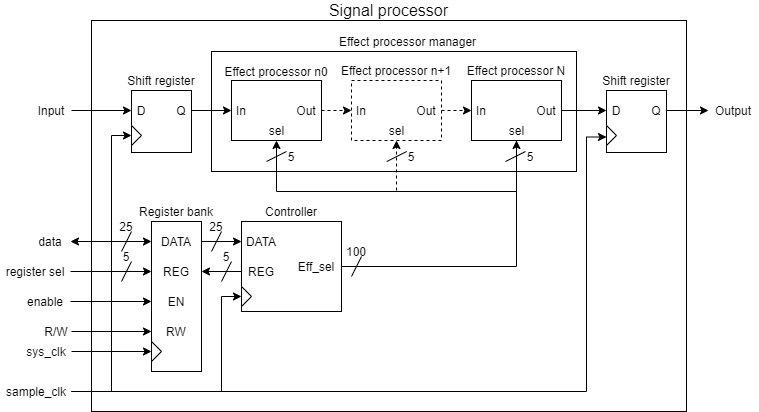
\includegraphics[width=\linewidth]{Signal processor architecture}
    \caption{Signal processor architecture}
    \label{fig:arch-signal-processor}
\end{figure}

The signal processor has to load a new sample into the effect loop and the previous modified sample to the output on the sample frequency. The sample frequency of the Audio-DSP is 192kHz. This means that the signal processor has $\frac{1}{192 \cdot 10^3} \approx 5 \mu s$ to process the sample. With a clock of 50MHz the sample must be modified and loaded into the output within $\frac{50 \cdot 10^6}{192 \cdot 10^3}=260$ clock ticks.
% \textbf{!!!This could be different according to the new design I just made - 28/04/2023 Youri !!! }\\

When a sample has been loaded into the signal processor, it is fed into the effect processor manager (see \ref{fig:arch-signal-processor}). The effect processor manager houses multiple effects processor in series. The sample will go through these effect processors. Each effect processor can be configured to be a certain effect (see \ref{fig:arch-effect-processor}). Because the system has at least twenty effects, the amount of bits the selector needs is 5 bits.

Each effect modifies the signal by applying a transfer function to the sample. The variables in that transfer function are configured by the user via the user interface. Therefore the effect processors needs to get the variables from the controller block, which gets the variables from the register bank. After the sample has gone through all the effect processors the modified sample waits before it is shifted out of the signal processor. 


\begin{figure}[ht]
    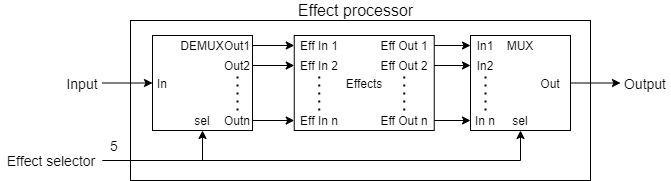
\includegraphics[width=\linewidth]{Effect processor architecture}
    \caption{Effect processor architecture}
    \label{fig:arch-effect-processor}
\end{figure}




    \chapter{Detailed Design}
    \section{Hardware Design}
    \input{hardware.tex}
    
    \section{Software Design}
    \input{software.tex}

    \chapter{System Interfaces}
    As described in the System Requirements Document (SRD), the audio DSP must include multiple input and output connectors and a user interface (UI).

\section{Inputs}
The system includes the following inputs:
\begin{itemize}
    \item DC jack to power the system
    \item CH1 RCA or jack
    \item CH2 RCA or jack
    \item CH3 XLR
    \item CH4 XLR
    \item CH5 USB (optional)
\end{itemize}
The USB input is optional and will only be added if we have sufficient time and the rest of the system is completed.

    \chapter{Human Machine Interface}
    \section{User interface}
A well-designed user interface is a critical component of any audio DSP project, particularly when utilizing a Nextion or similar screen. The user interface should be designed with simplicity in mind to ensure it is accessible to everyone who uses it. One of the primary goals of a good UI is to ensure that it is intuitive and easy to remember, so that users can begin using the product without feeling frustrated or overwhelmed.

\subsubsection*{Consistent}
The UI should maintain a consistent style throughout, so that each new menu or dial looks and feels the same as every other menu. This ensures that using the menus is easy and recognizable, even for new users.

\subsubsection*{Readability}
Text shown in menus should not be cut off, as this can be frustrating for users trying to read it. Short sentences are preferred to keep the menus clean and easy to read. When a sentence is cut off by the edge of the screen, users may struggle to figure out what it says, leading to confusion and frustration.

\subsubsection*{Feedback}
Finally, it is important to provide feedback to the user when the system needs time to load in certain elements or execute specific settings. Without feedback, users may become frustrated and begin clicking buttons multiple times, which can lead to software errors. By providing clear feedback during loading processes, users are more likely to remain patient and avoid potential issues.

\section{Designing the UI}
The design was started with a diagram with all the necessary screens and information so that is was clear what menus should be in the DSP. 

\begin{figure}[ht]
    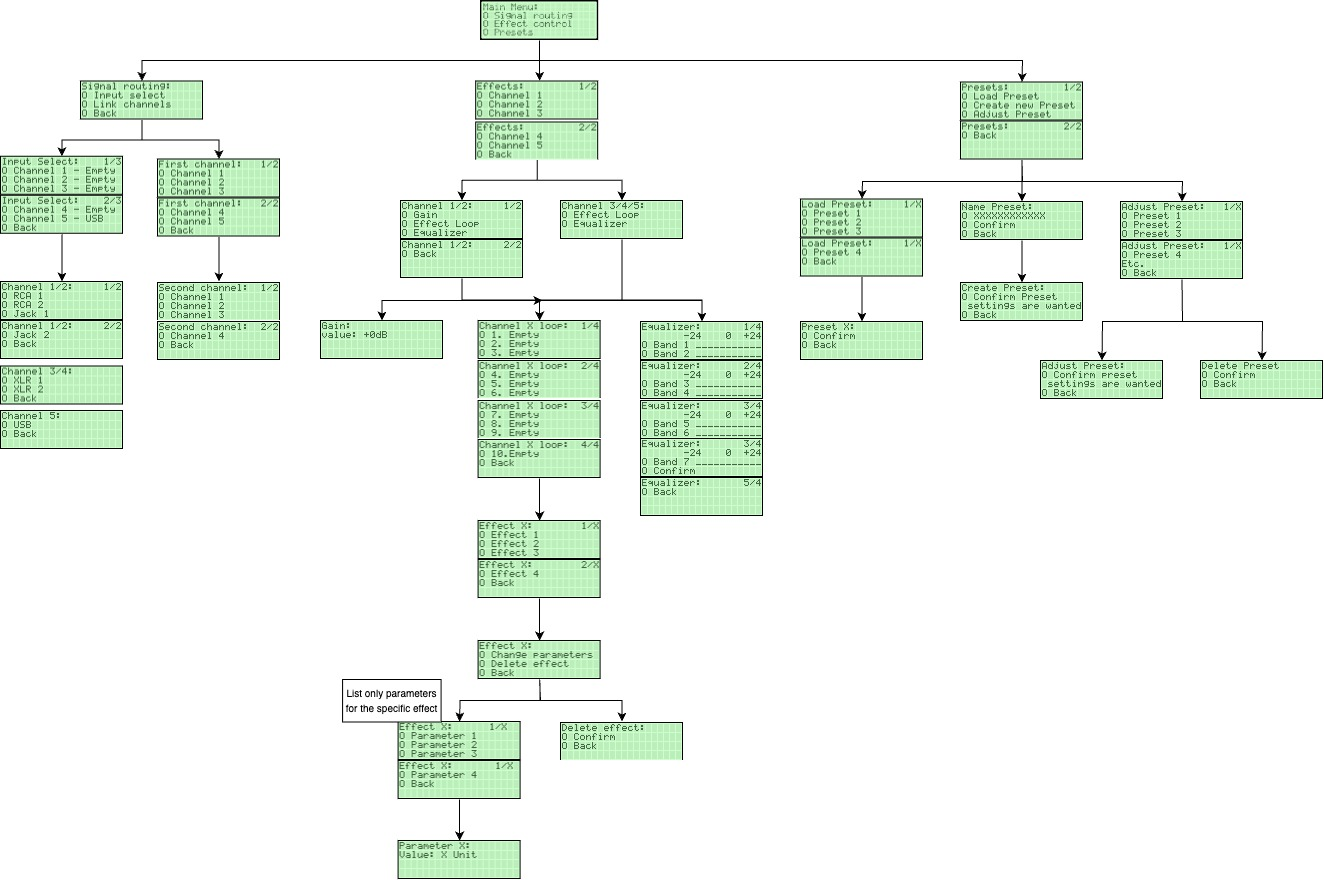
\includegraphics[width=\linewidth]{functionbasedUI}
    \caption{Function Based UI Design for a liquidCrystal screen}
    \label{fig:functionbasedUI}
\end{figure}

This UI is easy to understand when first using the DSP. Options and settings are easy to find from the first menu screen. While a channel based UI is unclear because every option is branched off from the channel select.

\section{Nextion screen}

For this project a Nextion screen is used. This screen can easily be programmed. It comes with software which is image based instead of code based. Images can be inserted and "invisible" buttons can be used to make menus out of the inserted images.

This is a neat way to work because now it is possible to create images in Photoshop or a similar application to use for the whole menu design.

    \end{justify}
\end{document}